\documentclass[11pt]{article}
\usepackage{amsmath}
\usepackage{gnuplottex}
\usepackage{geometry}
\usepackage{wrapfig}
\usepackage{float}
\usepackage{graphicx}
\usepackage[ngerman]{babel}
\usepackage{a4wide}
\usepackage{amsfonts}
\usepackage{enumerate}
\usepackage[utf8]{inputenc}
\setcounter{secnumdepth}{-1}
\geometry{a4paper, left=25mm, right=20mm, top=20mm, bottom=20mm}
\begin{document}

\begin{titlepage}
\title{Projektarbeit: Das Räuber-Beute-Modell \\ \small{pray-predator-model}\\ \includegraphics[scale=0.1]{Bilder/HaseLuxStat.png}}
\author{Tobias Möhle \\ 211204256}
\date{28.01.2013}
\maketitle
\end{titlepage}

\section{Einleitung}
Das Räuber-Beute-Modell ist ein Modell aus der Ökologie, welches das kleinste "okologische System beschreibt: zwei Populationen; eine Räuber- und eine Beutepopulation. Wie sich diese Populationen gegenseitig beeinflussen, bzw. wie sich dieser Einfluss beschreiben lässt, soll im Folgenden betrachtet werden.
Eine Betrachtungsweise ist ein deterministisches Modell, welches durch die Lotka-Volterra-Gleichungen\footnote{http://de.wikipedia.org/wiki/Lotka-Volterra-Gleichungen (am 25.01.2013)}
$$\dot x=x(k_1 A-k_{12}y)=0$$
$$\dot y=y(k_{21}x-k_2)=0$$
beschrieben wird.
Hierbei soll $x$ die Beute- und $y$ die Räuberpopulation darstellen. Die Parameter haben die Bedeutung
\begin{itemize}
   \item $k_1 A$ ist eine Größe, welche die Fertilität der Beutetiere beschreibt. Diese wird einerseits durch populationsspezifische Größen (Häufigkeit der Geburten, Anzahl der Kinder je Geburt etc.), welche in $k_1$ zusammengefasst sind, und andererseits durch die vorhandene Nahrungsmenge, symbolisiert mit $A$, beschrieben.
   \item $k_2$ beschreibt die Mortalität der Räuber
   \item $k_{21}$ und $k_{12}$ sind Größen, welche die Wechselwirkung der Populationen beschreibt, also die Anzahl der gerissenen Beutetiere auf der einen Seite und die Fertilität der Räuber auf der anderen Seite (welche von deren Nahrungsgrundlage, den Beutetieren, abhängt).
\end{itemize}

Die Lotka-Volterra-Gleichungen sind nicht allgemein lösbar, jedoch kann man an ihnen Betrachtungen zum Langzeit- und Stabilitätsverhalten durchführen.\\
Eine analoge Beschreibung wird durch die drei Reaktionsgleichungen 
$$x+A \xrightarrow{k_1} 2x $$
$$y \xrightarrow[k_{21}]{k_{12}} 0 $$
$$x+y \xrightarrow{k_2} 2y $$
gezeigt.
Ihr liegt, wie allen chemischen Prozessen, ein stochastisches Modell zu Grunde, welches mit Hilfe entsprechender Methoden analysiert werden kann. Eine Betrachtung durch die Master-Gleichung und eine Analyse mit Hilfe des Gillespie-Algorithmus' werden im folgenden vorgestellt.

\section{Deterministische Betrachtung}
Die deterministische Betrachtung des Räuber-Beute-Systems folgt, wie bereits oben erwähnt, mit den gekoppelten Differenzialgleichungen 1. Ordnung
$$\dot x=x(k_1 A-k_{12}y)=0$$
$$\dot y=y(k_{21}x-k_2)=0$$
Da diese analytisch nicht lösbar sind, werden hier lediglich die stationären Lösungen, das heißt Lösungen, bei welchen sich das System nicht mehr verändert und entsprechend Langzeitlösungen sind, betrachtet.\\
Im stationären Fall gilt entsprechend: $\dot x=\dot y=0$. Hieraus ergeben sich zwei stabile Punkte:
 $x_1=0$, $y_1=0$, $x_2=\frac{k_2}{k_{21}}$, $y_2=\frac{k_1 A}{k_{12}}$.\\
Nun gilt es, zu untersuchen, wie stabil das System gegenüber kleinen Schwankungen an diesen Punkten ist. Dies lässt sich mit der Gleichung
$\delta \begin{pmatrix} \dot x \\ \dot y \end{pmatrix}=J\delta \begin{pmatrix} x \\ y \end{pmatrix}$ wobei $J$ die Jakobimatrix ist:\\
$J=\begin{pmatrix} k_1A-k_{12}y & -k_{12}x \\ k_{21}y & k_{21}x-k_2 \end{pmatrix}$.\vspace{3mm} \\
untersuchen.\\
Für $x_1$, $y_1$ gilt also:
$\begin{vmatrix} k_1 A -\lambda & 0 \\ 0 & -k_2-\lambda \end{vmatrix}=(\lambda-k_1A)(\lambda+k_2)$.\\
Da alle Koeffizienten positiv sind, ist das System an dem Punkt, wo beide Populationen ausgestorben sind, instabil. An dieser Lösung wird deutlich, dass in dem Modell nicht nur Geburt, sondern auch Zuwanderung aus anderen Populationen zu einer Zunahme der Anzahl der Tiere möglich ist.
Für $x_2$, $y_2$ gilt:
$\begin{vmatrix} -\lambda & -k_{12}\frac{k_2}{k_21} \\ k_{21}\frac{k_1 A}{k_12} & -\lambda \end{vmatrix}=\lambda^2+k_1k_2A$.\\
Dieses System hat lediglich die imaginären Lösungen $\lambda=\pm i\sqrt{k_2k_1A}$. Rein imagiäre Lösungen beschreiben weder stabile noch instabile Systeme sondern ozillierende Lösungen (analog zu Schwingungsgleichungen in der Mechanik).\\
Es l"asst sich zeigen, dass, analog dem mathematischen Pendel oder anderen oszillierenden Systemen hier eine Erhaltungsgr"o\ss e analog der Energie bzw. Hamilton-Funktion eingef"uhrt werden kann\footnote{R. Mahnke \glqq Nichtlineare Physik in Aufgaben \grqq Verlag: B.G. Teubner, Stuttgart 1994; S. 125}. Diese lautet:
$$H=k_{21}x-k_2\ln(x)+k_{12}-k_1A\ln(y)=const$$

\section{Betrachtung mit der Master-Gleichung}
Das betrachtete System kann mit zwei unterschiedlichen Master-Gleichungen beschrieben werden: zum einen durch die diskrete Master-Gleichung
$$\frac{\partial}{\partial t} P(n, m, t)=k_1\,A (n-1) P(n-1, m, t) +k_{21}(n+1)(m-1) P(n+1, m-1, t)+k_2 (m+1) P(n, m+1, t)-$$ $$\left[ k_1 A n+ k_{21} n m +k_2 m \right] P(n,m,t)$$
bei welcher $n$ die Gr"o\ss e der Beute-Population und $m$ die der R"auber-Population ist. Diese l"asst sich nun in eine kontinuierliche Gleichung "uberf"uhren, indem man von einer maximalien Gesamtpopulation $V$ ausgeht, welche nicht "uberschritten werden kann. F"ur gro\ss e Populationen ($lim_{V \rightarrow \infty}$) wird das System kontinuierlich mit den Gr"oßen $x=\frac{n}{V}$, $y=\frac{m}{V}$. Nun gilt die Master-Gleichung: %Hier entsprechend erg"anzen!!!
Dies ist eine diskrete Master-Gleichung, welche auf Ein-Schritt-Prozesse beschränkt ist. Außerdem ist hier bereits die Vereinfachung gemacht, dass die Konstanten $k_{21}$ und $k_12$ als gleich angenommen werden.\\
Da jedoch zun"achst beliebig viele Tiere in beiden Populationen vorkommen k"onnen, stellt diese Gleichung ein System von unendlich vielen gekoppelten Differentialgleichungen dar. 

\section{Berechnungen mit dem Gillespie-Algorithmus}
Der Gillespie-Algorithmus untersucht stochastische Prozesse mit einem % experimentellen ////////////////////////////////////
Ansatz: Es werden eine Anzahl von Durchl"aufen des Prozesses mit Hilfe von Zufallsfunktionen berechnet und anschließend "uber diese gemittelt. Wurden genügend Durchläufe gemacht und sind die verwendeten Zufallsalgorithmen gut, so entsprechen die mit dem Gillespie-Algorithmus gewonnenen Ergebnisse denen der deterministischen Lösung. Das genaue Vorgehen beim Gillespie-Algorithmus lautet wie folgt\footnote{http://www.co-nan.eu/pdf/df2.pdf (28.01.2013) }:
\begin{enumerate}
   \item Initialisiere zun"achst alle Startwerte (Anfangsbedingungen, Konstanten etc).
   \item Generiere zwei Zufallszahlen $\tau$, $\rho$
   \item Nun wird das System erweitert: Aus den oben generierten Zufallszahlen wird ein Zeitschritt ermittelt, bei welchem der Prozess durchgef"uhrt wird, und aus der zweiten Zahl wird bestimmt, welcher der m"ogleichen Prozesse durchgef"uhrt wird. Nun m"ussen die jeweiligen Wahrscheinlichkeiten an die ver"anderten Zahlen angepasst werden.
   \item Ist die zu Beginn festgelegte Simulationsdauer noch nicht erreicht, beginne wieder bei Schritt 2.
\end{enumerate}

Mit Hilfe dieses Algorithmus' l"asst sich das R"auber-Beute-Modell nun sehr gut beschreiben. In einer Implementierung des Algorithmus' ergaben sich folgende Abl"aufe:

Hier exemplarisch zun"achst eine Einzeltrajektorie eines m"oglichen Prozesses:

\begin{figure}
\caption{Einzeltrajektorie des R"auber-Beute-Modells (mit Gillespie-Algorithmus berechnet)}
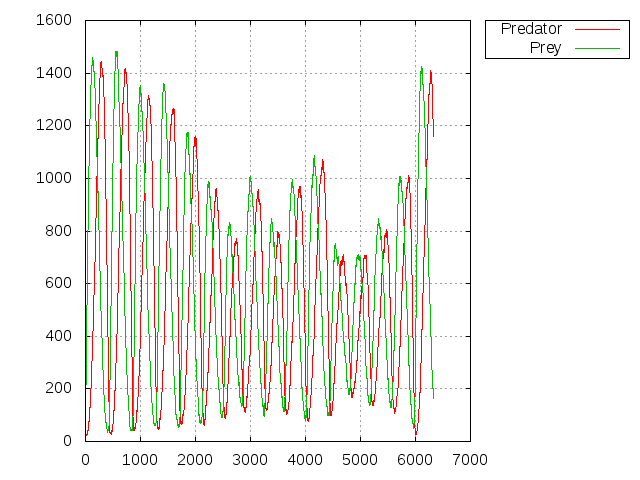
\includegraphics[scale=0.7]{Graphiken/ppm1_timepop.png}
\end{figure}

\end{document}
